%% LyX 2.3.6.2 created this file.  For more info, see http://www.lyx.org/.
%% Do not edit unless you really know what you are doing.
\documentclass[english,aspectratio=169,handout]{beamer}
\usepackage{mathptmx}
\usepackage{eulervm}
\usepackage[T1]{fontenc}
\usepackage[latin9]{inputenc}
\usepackage{babel}
\usepackage{amstext}
\usepackage{amssymb}
\usepackage{graphicx}
\ifx\hypersetup\undefined
  \AtBeginDocument{%
    \hypersetup{unicode=true,pdfusetitle,
 bookmarks=true,bookmarksnumbered=false,bookmarksopen=false,
 breaklinks=false,pdfborder={0 0 0},pdfborderstyle={},backref=false,colorlinks=true,
 allcolors=NYUPurple,urlcolor=LightPurple}
  }
\else
  \hypersetup{unicode=true,pdfusetitle,
 bookmarks=true,bookmarksnumbered=false,bookmarksopen=false,
 breaklinks=false,pdfborder={0 0 0},pdfborderstyle={},backref=false,colorlinks=true,
 allcolors=NYUPurple,urlcolor=LightPurple}
\fi

\makeatletter


%%%%%%%%%%%%%%%%%%%%%%%%%%%%%% LyX specific LaTeX commands.
%% Because html converters don't know tabularnewline
\providecommand{\tabularnewline}{\\}

%%%%%%%%%%%%%%%%%%%%%%%%%%%%%% Textclass specific LaTeX commands.
% this default might be overridden by plain title style
\newcommand\makebeamertitle{\frame{\maketitle}}%
% (ERT) argument for the TOC
\AtBeginDocument{%
  \let\origtableofcontents=\tableofcontents
  \def\tableofcontents{\@ifnextchar[{\origtableofcontents}{\gobbletableofcontents}}
  \def\gobbletableofcontents#1{\origtableofcontents}
}

%%%%%%%%%%%%%%%%%%%%%%%%%%%%%% User specified LaTeX commands.
\usetheme{CambridgeUS} 
\beamertemplatenavigationsymbolsempty


% Set Color ==============================
\definecolor{NYUPurple}{RGB}{87,6,140}
\definecolor{LightPurple}{RGB}{165,11,255}


\setbeamercolor{title}{fg=NYUPurple}
%\setbeamercolor{frametitle}{fg=NYUPurple}
\setbeamercolor{frametitle}{fg=NYUPurple}

\setbeamercolor{background canvas}{fg=NYUPurple, bg=white}
\setbeamercolor{background}{fg=black, bg=NYUPurple}

\setbeamercolor{palette primary}{fg=black, bg=gray!30!white}
\setbeamercolor{palette secondary}{fg=black, bg=gray!20!white}
\setbeamercolor{palette tertiary}{fg=gray!20!white, bg=NYUPurple}

\setbeamertemplate{headline}{}

\setbeamercolor{parttitle}{fg=NYUPurple}
\setbeamercolor{sectiontitle}{fg=NYUPurple}
\setbeamercolor{sectionname}{fg=NYUPurple}
\setbeamercolor{section page}{fg=NYUPurple}

\AtBeginSection[]{
  \begin{frame}
    \frametitle{Table of Contents}
    \tableofcontents[currentsection]
  \end{frame}

  % \begin{frame}
  % \vfill
  % \centering
  % \begin{beamercolorbox}[sep=8pt,center,shadow=true,rounded=true]{title}
  %   \usebeamerfont{title}\insertsectionhead\par%
  % \end{beamercolorbox}
  % \vfill
  % \end{frame}
}

\makeatother

\begin{document}
\global\long\def\reals{\mathbf{R}}%
 
\global\long\def\integers{\mathbf{Z}}%
 
\global\long\def\naturals{\mathbf{N}}%
 
\global\long\def\rationals{\mathbf{Q}}%
 
\global\long\def\ca{\mathcal{A}}%
 
\global\long\def\cb{\mathcal{B}}%
 
\global\long\def\cc{\mathcal{C}}%
 
\global\long\def\cd{\mathcal{D}}%
 
\global\long\def\ce{\mathcal{E}}%
 
\global\long\def\cf{\mathcal{F}}%
 
\global\long\def\cg{\mathcal{G}}%
 
\global\long\def\ch{\mathcal{H}}%
 
\global\long\def\ci{\mathcal{I}}%
 
\global\long\def\cj{\mathcal{J}}%
 
\global\long\def\ck{\mathcal{K}}%
 
\global\long\def\cl{\mathcal{L}}%
 
\global\long\def\cm{\mathcal{M}}%
 
\global\long\def\cn{\mathcal{N}}%
 
\global\long\def\co{\mathcal{O}}%
 
\global\long\def\cp{\mathcal{P}}%
 
\global\long\def\cq{\mathcal{Q}}%
 
\global\long\def\calr{\mathcal{R}}%
 
\global\long\def\cs{\mathcal{S}}%
 
\global\long\def\ct{\mathcal{T}}%
 
\global\long\def\cu{\mathcal{U}}%
 
\global\long\def\cv{\mathcal{V}}%
 
\global\long\def\cw{\mathcal{W}}%
 
\global\long\def\cx{\mathcal{X}}%
 
\global\long\def\cy{\mathcal{Y}}%
 
\global\long\def\cz{\mathcal{Z}}%
 
\global\long\def\ind#1{1(#1)}%
 %\newcommand{\pr}{P}
\global\long\def\pr{\mathbb{P}}%
 
\global\long\def\predsp{\cy}%
 %{\hat{\cy}}
\global\long\def\outsp{\cy}%

\global\long\def\prxy{P_{\cx\times\cy}}%
 
\global\long\def\prx{P_{\cx}}%
 
\global\long\def\prygivenx{P_{\cy\mid\cx}}%
 %\newcommand{\ex}{E}
\global\long\def\ex{\mathbb{E}}%
 
\global\long\def\var{\textrm{Var}}%
 
\global\long\def\cov{\textrm{Cov}}%
 
\global\long\def\sgn{\textrm{sgn}}%
 
\global\long\def\sign{\textrm{sign}}%
 
\global\long\def\kl{\textrm{KL}}%
 
\global\long\def\law{\mathcal{L}}%
 
\global\long\def\eps{\varepsilon}%
 
\global\long\def\as{\textrm{ a.s.}}%
 
\global\long\def\io{\textrm{ i.o.}}%
 
\global\long\def\ev{\textrm{ ev.}}%
 
\global\long\def\convd{\stackrel{d}{\to}}%
 
\global\long\def\eqd{\stackrel{d}{=}}%
 
\global\long\def\del{\nabla}%
 
\global\long\def\loss{\ell}%
 
\global\long\def\risk{R}%
 
\global\long\def\emprisk{\hat{R}}%
 
\global\long\def\lossfnl{L}%
 
\global\long\def\emplossfnl{\hat{L}}%
 
\global\long\def\empminimizer#1{\hat{#1}^{*}}%
 
\global\long\def\minimizer#1{#1^{*}}%
\global\long\def\optimizer#1{#1^{*}}%
 
\global\long\def\etal{\textrm{et. al.}}%
 
\global\long\def\tr{\operatorname{tr}}%

\global\long\def\trace{\operatorname{trace}}%
 
\global\long\def\diag{\text{diag}}%
 
\global\long\def\rank{\text{rank}}%
 
\global\long\def\linspan{\text{span}}%
 
\global\long\def\spn{\text{span}}%
 
\global\long\def\proj{\text{Proj}}%
 
\global\long\def\argmax{\operatornamewithlimits{arg\, max}}%
 
\global\long\def\argmin{\operatornamewithlimits{arg\, min}}%

\global\long\def\bfx{\mathbf{x}}%
 
\global\long\def\bfy{\mathbf{y}}%
 
\global\long\def\bfl{\mathbf{\lambda}}%
 
\global\long\def\bfm{\mathbf{\mu}}%
 
\global\long\def\calL{\mathcal{L}}%

\global\long\def\vw{\boldsymbol{w}}%
 
\global\long\def\vx{\boldsymbol{x}}%
 
\global\long\def\vxi{\boldsymbol{\xi}}%
 
\global\long\def\valpha{\boldsymbol{\alpha}}%
 
\global\long\def\vbeta{\boldsymbol{\beta}}%
 
\global\long\def\vsigma{\boldsymbol{\sigma}}%
\global\long\def\vtheta{\boldsymbol{\theta}}%
 
\global\long\def\vd{\boldsymbol{d}}%
 
\global\long\def\vs{\boldsymbol{s}}%
 
\global\long\def\vt{\boldsymbol{t}}%
 
\global\long\def\vh{\boldsymbol{h}}%
 
\global\long\def\ve{\boldsymbol{e}}%
 
\global\long\def\vf{\boldsymbol{f}}%
 
\global\long\def\vg{\boldsymbol{g}}%
 
\global\long\def\vz{\boldsymbol{z}}%
 
\global\long\def\vk{\boldsymbol{k}}%
 
\global\long\def\va{\boldsymbol{a}}%
 
\global\long\def\vb{\boldsymbol{b}}%
 
\global\long\def\vv{\boldsymbol{v}}%
 
\global\long\def\vy{\boldsymbol{y}}%

\global\long\def\dom{\textrm{\textbf{dom} }}%
\global\long\def\rank{\text{\textbf{rank }}}%
\global\long\def\conv{\textrm{\textbf{conv} }}%
\global\long\def\relint{\text{\textbf{relint }}}%
\global\long\def\aff{\text{\textbf{aff }}}%

\global\long\def\hil{\ch}%
 
\global\long\def\rkhs{\hil}%
 
\global\long\def\ber{\text{Ber}}%

\global\long\def\softmax{\text{Softmax}}%

\title[DS-GA 1003 ]{Probabilistic models\\
- \\
Maximum Likelihood Estimation}
\author{Marylou Gabri\'e
\\
\vspace{1cm}
Slides based on Lecture \href{https://github.com/davidrosenberg/mlcourse/blob/gh-pages/Lectures/06b.MLE.pdf}{06b} from David Rosenberg's course materials (\url{https://github.com/davidrosenberg/mlcourse})}
\date{March 9, 2021}
\institute{CDS, NYU}

\makebeamertitle
\mode<article>{Just in article version}

\begin{frame}{The Data: Assumptions So Far in this Course}
  \begin{itemize}
  \item Our usual setup is that $(x,y)$ pairs are drawn {\bf i.i.d. from $\cp_{\cx\times\cy}$}.
  \pause{}
  \item So far ridge/lasso/
  regression, optimization, SVMs, and kernel methods are applicable for arbitrary
  training data sets $\cd:\left(x_{1},y_{1}\right),\ldots,\left(x_{n},y_{n}\right)\in\cx\times\cy$.
  \begin{itemize}
  \item i.e. $\cd$ could be created by hand, by an adversary, or randomly.
  
  \pause{}
  \end{itemize}

  \pause{}
  \item How have we used this assumption so far?
  
  \pause{}
  \begin{itemize}
  \item motivates empirical risk minimization 
  
  \item ties test performance to performance on new data when deployed
  \pause{}
  \end{itemize}
  
  \item We rely on the i.i.d. $\cp_{\cx\times\cy}$ assumption when it comes
  to \textbf{generalization} only.
  \end{itemize}
\end{frame}

\begin{frame}{Probabilistic Models: Use Assumptions on the Data for Learning}

\begin{itemize}
  \item Observations $y$ are drawn i.i.d. from a distribution $\cp_{\cy}$  \\
  $\rightarrow$ {\bf Maximum likelihood estimation} (First topic of week 6)
  \pause{}
  \item Model how $y$ depends on $x$  \\
  $\rightarrow$ {\bf Conditional probability models} $p(y|x)$ (Second topic of week 6)
  \pause{}
  \item Incorporate prior knowledge and estimate uncertainty on the prediction\\
  $\rightarrow$ {\bf Bayesian approaches} (Topic of week 7)  
\end{itemize}
  
\end{frame}

\begin{frame}{Maximum Likelihood Estimation: Contents}

\tableofcontents{}
\end{frame}


\section{Likelihood of an Estimated Probability Distribution}
\begin{frame}{Estimating a Probability Distribution: Setting}
For the moment we only assume that we have one variable $y$.
\begin{itemize}
\item Let $p(y)$ represent a probability distribution on $\cy$.
\item $p(y)$ is \textbf{unknown} and we want to \textbf{estimate} it.

\pause{}
\item Assume that $p(y)$ is either a
\begin{itemize}
\item probability density function on a continuous space $\cy$, or a
\item probability mass function on a discrete space $\cy$.

\pause{}
\end{itemize}
\item Typical $\cy$'s:
\begin{itemize}
\item $\cy=\reals$; $\cy=\reals^{d}$ {[}typical continuous distributions{]}
\item $\cy=\left\{ -1,1\right\} $ {[}e.g. binary classification{]}
\item $\cy=\left\{ 0,1,2,\ldots,K\right\} $ {[}e.g. multiclass problem{]}
\item $\cy=\left\{ 0,1,2,3,4\ldots\right\} $ {[}unbounded counts{]}
\end{itemize}
\end{itemize}
\end{frame}

\begin{frame}{Evaluating a Probability Distribution Estimate}

\begin{itemize}
\item Before we talk about estimation, let's talk about evaluation.

\pause{}
\item Somebody gives us an estimate of the probability distribution
\[
\hat{p}(y).
\]
\item How can we evaluate how good it is?

\pause{}
\item We want $\hat{p}(y)$ to be descriptive of \textbf{future} data. 

\end{itemize}
\end{frame}

\begin{frame}{Likelihood of a Predicted Distribution}

\begin{itemize}
\item Suppose we have
\[
\cd=\left(y_{1},\ldots,y_{n}\right)\text{ sampled i.i.d. from true distribution }p(y).
\]
\item Then the \textbf{likelihood }of $\hat{p}$ for the data $\cd$ is
defined to be
\[
\hat{p}(\cd)=\prod_{i=1}^{n}\hat{p}(y_{i}).
\]
\center
The probability of observing $\cd$ under the estimate $\hat{p}$.

\pause{}
\item How are we going to construct an estimate of $\hat{p}(y)$?
\end{itemize}
\end{frame}

\section{Parametric Families of Distributions}
\begin{frame}{Parametric Models}
\begin{definition}
A \textbf{parametric model }is a set of probability distributions
indexed by a parameter $\theta\in\Theta$. We denote this as
\[
\left\{ p(y;\theta)\mid\theta\in\Theta\right\} ,
\]
where $\theta$ is the \textbf{parameter} and $\Theta$ is the \textbf{parameter
space}.

\pause{}
\end{definition}

\begin{itemize}
\item Below we'll give some examples of common parametric models.
\begin{itemize}
\item But it's worth doing research to find a parametric model most appropriate
for your data. 
\end{itemize}

\pause{}
\item We'll sometimes say\textbf{ family of distributions} for a probability
model.
\end{itemize}

\end{frame}

\begin{frame}{Poisson Family}
\begin{columns}[t]

\column{.6\textwidth}
\begin{itemize}
\item Support $\cy=\left\{ 0,1,2,3,\ldots\right\} $.
\item Parameter space: $\left\{ \lambda\in\reals\mid\lambda>0\right\} $
\item Probability mass function on $k\in\cy$:
\[
p(k;\lambda)=\lambda^{k}e^{-\lambda}/\left(k!\right)
\]
\end{itemize}

% \pause{}

\column{.35\textwidth}
\begin{center}
\includegraphics[width=1\columnwidth]{../../drosenberg-mlcourse-archive/Archive/2019/Lectures/source/05c.MLE/poissonDistribution}
\par\end{center}

\end{columns}

\pause{}
\begin{itemize}
  \item Examples: Number of random i.i.d. events in a given time/over an interval
  \begin{itemize}
    \item Radioactive decay of atoms over a year
    \item Number of taxi cab pickups at Penn Station in an evening
  \end{itemize}
\end{itemize}

\let\thefootnote\relax\footnotetext{\tiny{Figure is "Poisson pmf" by Skbkekas - Own work. Licensed under CC BY 3.0 via Wikimedia Commons - \url{http://commons.wikimedia.org/wiki/File:Poisson_pmf.svg\#/media/File:Poisson_pmf.svg}.}}
\end{frame}
%
\begin{frame}{Beta Family}
\begin{columns}[t]

\column{.6\textwidth}
\begin{itemize}
\item Support $\cy=(0,1)$. {[}The unit interval.{]}
\item Parameter space: $\left\{ \theta=\left(\alpha,\beta\right)\mid\alpha,\beta>0\right\} $
\item Probability density function on $y\in\cy$:
\[
p(y;a,b)=\frac{y^{\alpha-1}\left(1-y\right)^{\beta-1}}{B(\alpha,\beta)}
\]
\end{itemize}


\column{.35\textwidth}
\begin{center}
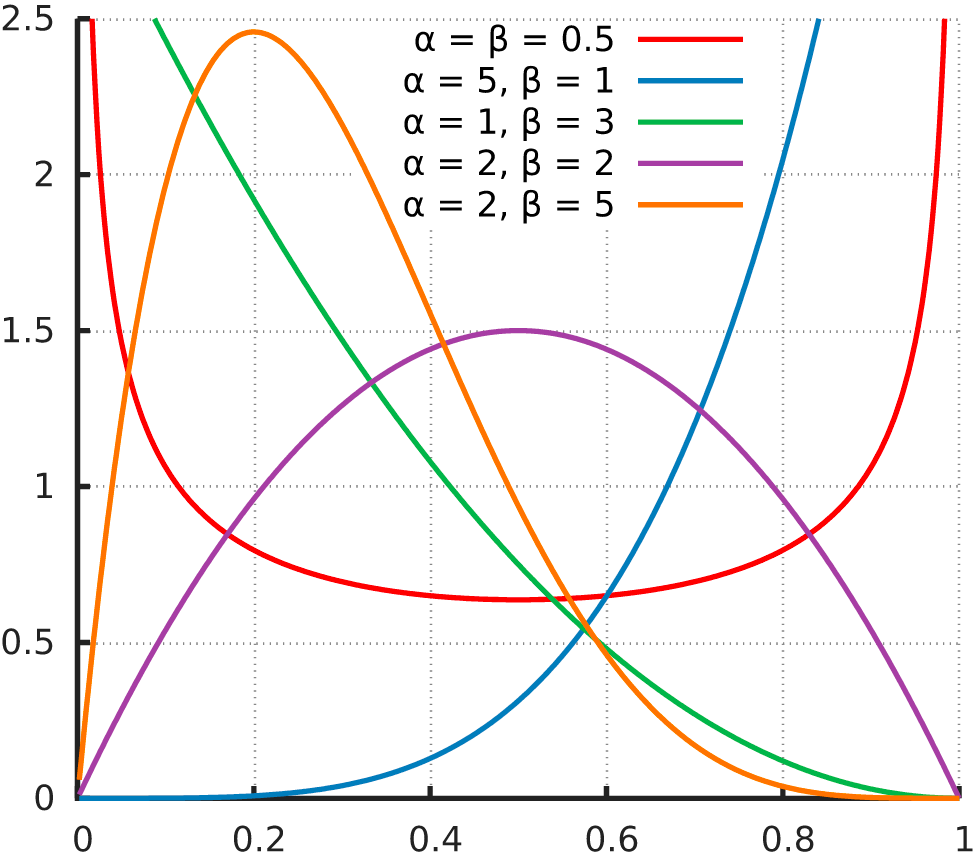
\includegraphics[width=0.9\columnwidth]{../../drosenberg-mlcourse-archive/Archive/2019/Lectures/source/05c.MLE/betaFamily}
\par\end{center}

\end{columns}

\pause{}
\begin{itemize}
  \item Examples: Spending of a resource over a interval.
  \begin{itemize}
    \item Project management
  \end{itemize}
\end{itemize}


\let\thefootnote\relax\footnotetext{\tiny{Figure by Horas based on the work of Krishnavedala (Own work) [Public domain], via \href{https://en.wikipedia.org/wiki/File:Beta_distribution_pdf.svg}{Wikimedia Commons}.}}
\end{frame}
%
% \begin{frame}{Gamma Family}
% \begin{columns}[t]

% \column{.6\textwidth}
% \begin{itemize}
% \item Support $\cy=(0,\infty)$. {[}Positive real numbers{]}
% \item Parameter space: $\left\{ \theta=\left(k,\theta\right)\mid k>0,\theta>0\right\} $ 
% \item Probability density function on $y\in\cy$:
% \[
% p(y;k,\theta)=\frac{1}{\Gamma(k)\theta^{k}}x^{k-1}e^{-y/\theta}.
% \]
% \end{itemize}

% \column{.35\textwidth}
% \begin{center}
% \includegraphics[width=0.9\columnwidth]{../../drosenberg-mlcourse-archive/Archive/2019/Lectures/source/05c.MLE/gammaFamily}
% \par\end{center}
% \end{columns}


% \pause{}
% \begin{itemize}
% \item Special cases: exponential distribution, chi-squared distribution,
% Erlang distribution
% \end{itemize}
% \let\thefootnote\relax\footnotetext{\tiny{Figure from Wikipedia \url{https://commons.wikimedia.org/wiki/File:Gamma_distribution_pdf.svg}.}}
% \end{frame}

\begin{frame}{Gaussian Family}
\begin{columns}[t]

\column{.6\textwidth}
\begin{itemize}
\item Support $\cy \in \reals$. 
\item Parameter space: $\left\{ \theta=\left(\mu,\sigma^2\right)\mid \mu \in \reals,\sigma^2>0\right\} $ 
\item Probability density function on $y\in\cy$:
\[
p(y;\mu,\sigma)=\frac{1}{\sqrt{2 \pi} \sigma}e^{-(y - \sigma)^2/2 \sigma^2}.
\]
\item Also named "normal" distribution, noted $\cn(\mu, \sigma^2)$
\end{itemize}

\column{.4\textwidth}
\begin{center}
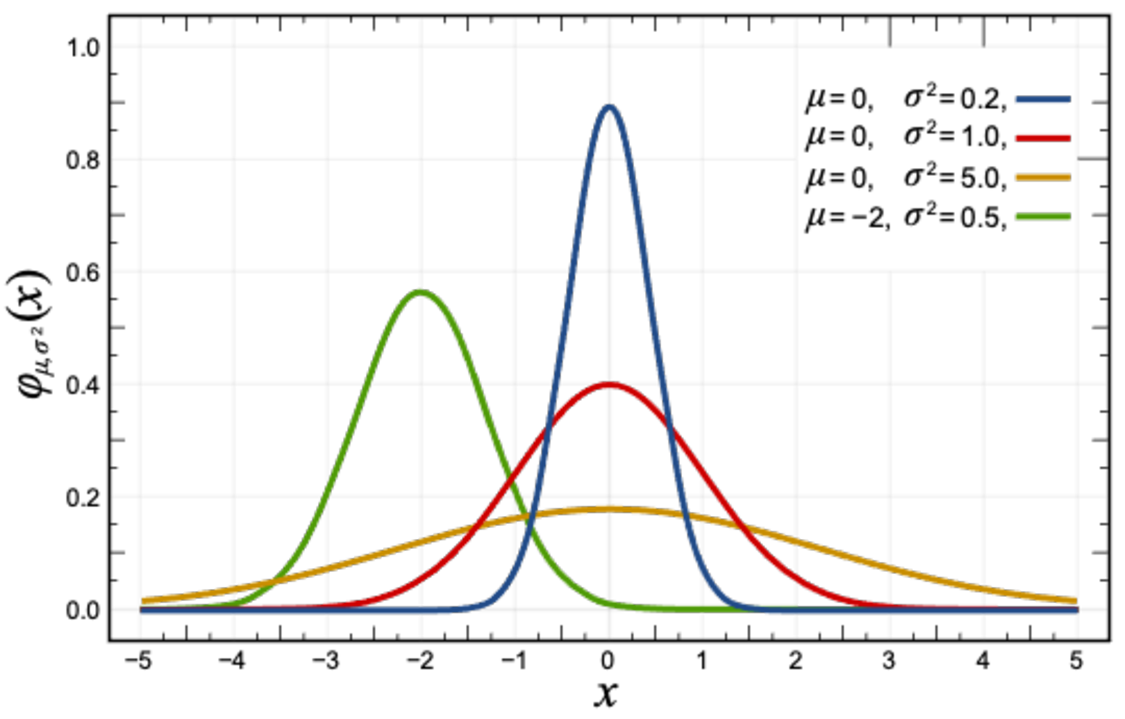
\includegraphics[width=0.99\columnwidth]{figs/6a_Normal_Distribution_PDF.pdf}
\par\end{center}
\end{columns}


\pause{}
\begin{itemize}
\item Examples: sum of i.i.d random variables (Central limit theorem)
  \begin{itemize}
    \item Cumulated gain from random independent coin flips
  \end{itemize}
\end{itemize}
\let\thefootnote\relax\footnotetext{\tiny{Figure from Wikipedia \url{https://en.wikipedia.org/wiki/Gaussian_function}.}}
\end{frame}

\begin{frame}{Multivariate Distributions}
  \begin{itemize}
    \item Above we only cited examples of univariate distributions
    \item Sometimes we need multivariate distributions $p(y; \theta)$ for $y = (y_1, \cdots, y_d)\in\reals^d$: 
    \begin{itemize}
      \item If $y_i$s are independent $p(y; \theta) = \prod_{i=1}^d p(y_i ;\theta_i)$
      \item If there are correlations, we have to treat the problem in dimension $d$.
    \end{itemize}
  \end{itemize}
  \begin{columns}[t]
  \column{.5\textwidth}
  \begin{itemize}
    \item Example: \\ Multivariate Gaussian Distribution
    \begin{itemize}
      \item In 2d: $y\in \reals^2$, $p(y; \theta) = \cn(\mu; \Sigma)$
      \item Parameters:\\
      \quad - Mean vector $\mu \in \reals^2$ \\
      \quad - Covariance matrix $\Sigma \in \reals^{2\times2}$
    \end{itemize}
  \end{itemize}
  \column{.45\textwidth}
  \begin{center}
    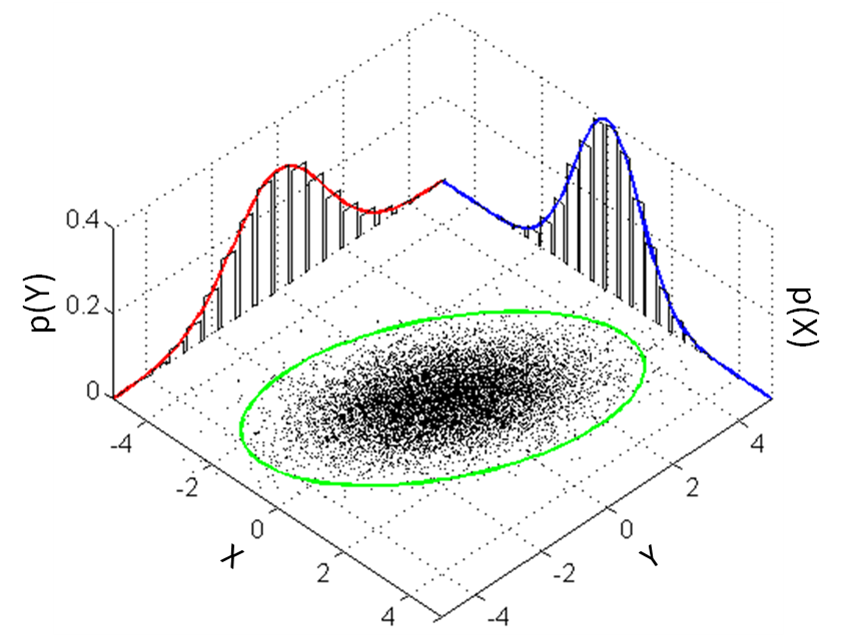
\includegraphics[width=0.8\columnwidth]{figs/6a_MultivariateNormal.png}
    \par\end{center}
  \end{columns}

\let\thefootnote\relax\footnotetext{\tiny{Figure from Wikipedia \url{https://en.wikipedia.org/wiki/Gaussian_function}.}}
\end{frame}


\section{Maximum Likelihood Estimation}
\begin{frame}{Likelihood in a Parametric Model}

Suppose we have a parametric model $\left\{ p(y;\theta)\mid\theta\in\Theta\right\} $
and a sample $\cd=\left(y_{1},\ldots,y_{n}\right)$.

\pause{}
\begin{itemize}
\item The \textbf{likelihood }of parameter estimate $\hat{\theta}\in\Theta$
for sample $\cd$ is
\[
p(\cd;\hat{\theta})\pause=\prod_{i=1}^{n}p(y_{i};\hat{\theta}).
\]
\end{itemize}

\pause{}
\begin{itemize}
\item In practice, we prefer to work with the \textbf{log-likelihood}. Same
maximizer, but
\[
\log p(\cd;\hat{\theta})=\sum_{i=1}^{n}\log p(y_{i};\hat{\theta}),
\]
and sums are easier to work with than products.
\end{itemize}
\end{frame}
%
\begin{frame}{Maximum Likelihood Estimation}
\begin{itemize}
\item Suppose $\cd=\left(y_{1},\ldots,y_{n}\right)$ is an i.i.d. sample
from some distribution. 
\end{itemize}
\begin{definition}
A \textbf{maximum likelihood estimator (MLE)} for $\theta$ in the
model $\left\{ p(y;\theta)\mid\theta\in\Theta\right\} $ is
\begin{eqnarray*}
\hat{\theta} & \in & \argmax_{\theta\in\Theta}\log p(\cd,\hat{\theta})\\
\pause & = & \argmax_{\theta\in\Theta}\sum_{i=1}^{n}\log p(y_{i};\theta).
\end{eqnarray*}
\end{definition}

\end{frame}
%
\begin{frame}{Maximum Likelihood Estimation}
\begin{itemize}
\item Finding the MLE is an \textbf{optimization problem}.
\end{itemize}

\pause{}
\begin{itemize}
\item For some model families, calculus gives a closed form for the MLE.
\end{itemize}

\pause{}
\begin{itemize}
\item Can also use numerical methods we know (e.g. SGD). 
\end{itemize}
\end{frame}
%
\begin{frame}{MLE Existence}
\begin{itemize}
\item In certain situations, the MLE may not exist. 
\item But there is usually a good reason for this.
\end{itemize}

\pause{}
\begin{itemize}
\item e.g. Gaussian family $\left\{ \cn(\mu,\sigma^{2})\mid\mu\in\reals,\sigma^{2}>0\right\} $
\item We have a single observation $y$. 
\item Is there an MLE?
\end{itemize}

\pause{}
\begin{itemize}
\item Taking $\mu=y$ and $\sigma^{2}\to0$ drives likelihood to infinity. 
\item MLE doesn't exist.
\end{itemize}
\end{frame}
%
\begin{frame}{Example: MLE for Poisson}
\begin{itemize}
\item Observed counts $\cd=\left(k_{1},\ldots,k_{n}\right)$ for taxi cab
pickups over $n$ weeks.
\begin{itemize}
\item $k_{i}$ is number of pickups at Penn Station Mon, 7-8pm, for week
$i$.
\end{itemize}
\item We want to fit a Poisson distribution to this data.

\pause{}
\item The Poisson log-likelihood for a single count is
\begin{eqnarray*}
\log\left[p(k;\lambda)\right] & = & \log\left[\frac{\lambda^{k}e^{-\lambda}}{k!}\right]\\
 & = & k\log\lambda-\lambda-\log\left(k!\right)
\end{eqnarray*}


\pause{}
\item The full log-likelihood is
\begin{eqnarray*}
\log p(\cd,\lambda) & = & \sum_{i=1}^{n}\left[k_{i}\log\lambda-\lambda-\log\left(k_{i}!\right)\right].
\end{eqnarray*}
 
\end{itemize}
\end{frame}

\begin{frame}{Example: MLE for Poisson}

\begin{itemize}
\item The full log-likelihood is
\begin{eqnarray*}
\log p(\cd,\lambda) & = & \sum_{i=1}^{n}\left[k_{i}\log\lambda-\lambda-\log\left(k_{i}!\right)\right]
\end{eqnarray*}


\pause{}
\item First order condition gives
\begin{eqnarray*}
0=\frac{\partial}{\partial\lambda}\left[\log p(\cd,\lambda)\right] & = & \sum_{i=1}^{n}\left[\frac{k_{i}}{\lambda}-1\right]\\
\pause\implies\lambda & = & \frac{1}{n}\sum_{i=1}^{n}k_{i}
\end{eqnarray*}


\pause{}
\item So MLE $\hat{\lambda}$ is just the mean of the counts. 
\end{itemize}
\end{frame}

\begin{frame}{Estimating Distributions, Overfitting, and Hypothesis Spaces}

\begin{itemize}
\item Just as in classification and regression, MLE can overfit! 

\pause{}
\item Example Probability Models: Penn Station, Mon-Fri 7-8pm
\begin{itemize}
\item $\cf=\left\{ \text{Poisson distributions}\right\} $.
\item $\cf=\left\{ \text{Negative binomial distributions}\right\} $.

\pause{}
\end{itemize}
\item How to judge which model works the best?

\pause{}
\item Choose the model with the \textbf{highest likelihood on validation
set}.
\pause{}
\begin{itemize}
  \item Test Set Log Likelihood for Penn Station, Mon-Fri 7-8pm
\end{itemize}
\end{itemize}
\begin{center}
\begin{tabular}{|c|c|}
\hline 
Method  & Test Log-Likelihood\tabularnewline
\hline 
\hline 
Poisson & $-392.16$\tabularnewline
\hline 
\textbf{Negative Binomial} & $-188.67$\tabularnewline
\hline 
\end{tabular}
\par\end{center}
  
\end{frame}

\end{document}
